\documentclass[12pt]{article}
\usepackage{amsfonts, amssymb, amsmath, amsthm}
\usepackage[margin=1in]{geometry}
\usepackage{tikz}
\usetikzlibrary{patterns, decorations.pathreplacing}

\pagestyle{myheadings}
\markright{Explainer: Rudin 4.23 --- Convex Functions\hfill}

\newcommand{\R}{\mathbb{R}}
\newcommand{\eps}{\varepsilon}

\begin{document}

\begin{center}
    \textbf{\Large Convex Functions: Continuity and Slope Inequalities}\\[0.5em]
    \large A visual guide to Rudin 4.23
\end{center}

\section{What Does Convex Mean?}

A function $f$ on $(a,b)$ is \textbf{convex} if for any two points, the chord lies above the curve:
\[
f(\lambda x + (1 - \lambda)y) \leq \lambda f(x) + (1 - \lambda)f(y) \quad \text{for } 0 < \lambda < 1
\]

\begin{center}
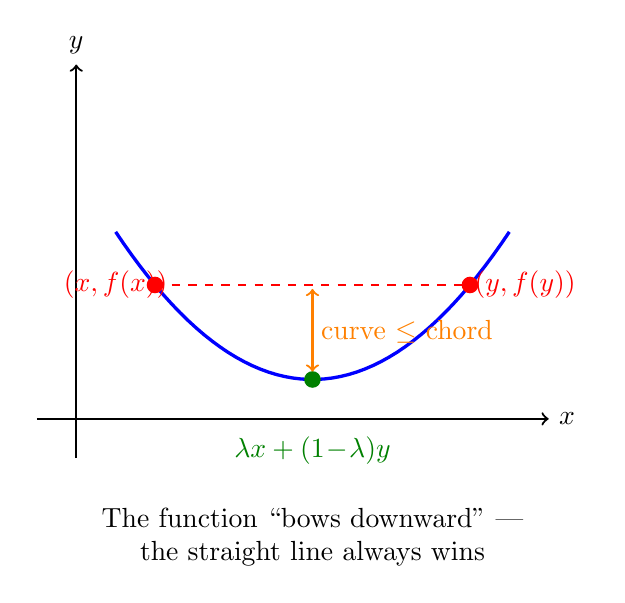
\begin{tikzpicture}[scale=1]
    \draw[thick, ->] (-0.5, 0) -- (6, 0) node[right] {$x$};
    \draw[thick, ->] (0, -0.5) -- (0, 4.5) node[above] {$y$};

    % Convex function
    \draw[blue, very thick, domain=0.5:5.5, samples=50] plot (\x, {0.3*(\x - 3)*(\x - 3) + 0.5});

    % Two points
    \fill[red] (1, {0.3*4 + 0.5}) circle (3pt);
    \fill[red] (5, {0.3*4 + 0.5}) circle (3pt);
    \node[red] at (0.5, 1.7) {$(x, f(x))$};
    \node[red] at (5.7, 1.7) {$(y, f(y))$};

    % Chord
    \draw[red, thick, dashed] (1, {0.3*4 + 0.5}) -- (5, {0.3*4 + 0.5});

    % A point on the chord vs curve
    \fill[green!50!black] (3, {0.3*0 + 0.5}) circle (3pt);
    \node[green!50!black] at (3, -0.4) {$\lambda x + (1\!-\!\lambda)y$};

    \draw[<->, orange, thick] (3, 0.6) -- (3, 1.65);
    \node[orange] at (4.2, 1.1) {curve $\leq$ chord};

    \node[text width=7cm, align=center] at (3, -1.5) {The function ``bows downward'' ---\\the straight line always wins};
\end{tikzpicture}
\end{center}

\section{Part 1: The Secant Slope Inequality}

If $a < s < t < u < b$, then:
\[
\frac{f(t) - f(s)}{t - s} \leq \frac{f(u) - f(s)}{u - s} \leq \frac{f(u) - f(t)}{u - t}
\]

In words: \textbf{secant slopes increase as you move right}.

\begin{center}
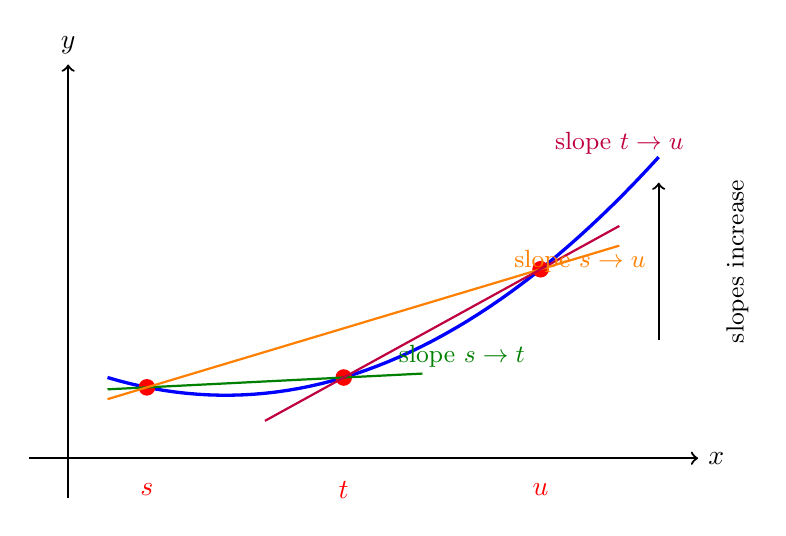
\begin{tikzpicture}[scale=1]
    \draw[thick, ->] (-0.5, 0) -- (8, 0) node[right] {$x$};
    \draw[thick, ->] (0, -0.5) -- (0, 5) node[above] {$y$};

    % Convex curve
    \draw[blue, very thick, domain=0.5:7.5, samples=50] plot (\x, {0.1*(\x - 2)*(\x - 2) + 0.8});

    % Three points
    \fill[red] (1, {0.1*1 + 0.8}) circle (3pt);
    \fill[red] (3.5, {0.1*2.25 + 0.8}) circle (3pt);
    \fill[red] (6, {0.1*16 + 0.8}) circle (3pt);

    \node[red] at (1, -0.4) {$s$};
    \node[red] at (3.5, -0.4) {$t$};
    \node[red] at (6, -0.4) {$u$};

    % Three secant lines
    \draw[green!50!black, thick] (0.5, {0.9 - 0.5*(1.025 - 0.9)/(2.5)}) -- (4.5, {0.9 + 3.5*(1.025 - 0.9)/(2.5)});
    \draw[orange, thick] (0.5, {0.9 - 0.5*(2.4 - 0.9)/5}) -- (7, {0.9 + 6*(2.4 - 0.9)/5});
    \draw[purple, thick] (2.5, {1.025 - 1*(2.4 - 1.025)/2.5}) -- (7, {1.025 + 3.5*(2.4 - 1.025)/2.5});

    % Legend
    \node[green!50!black] at (5, 1.3) {\small slope $s \to t$};
    \node[orange] at (6.5, 2.5) {\small slope $s \to u$};
    \node[purple] at (7, 4) {\small slope $t \to u$};

    \draw[->, thick] (7.5, 1.5) -- (7.5, 3.5);
    \node at (8.5, 2.5) {\rotatebox{90}{\small slopes increase}};
\end{tikzpicture}
\end{center}

\subsection{Why?}

Write $t$ as a convex combination of $s$ and $u$:
\[
t = \lambda s + (1 - \lambda) u \quad \text{where } \lambda = \frac{u - t}{u - s}
\]
Convexity gives $f(t) \leq \lambda f(s) + (1 - \lambda) f(u)$, which rearranges to the slope inequality.

\section{Part 2: Every Convex Function is Continuous}

This is surprising --- convexity is an \emph{algebraic} condition, but it forces \emph{topological} regularity!

\begin{center}
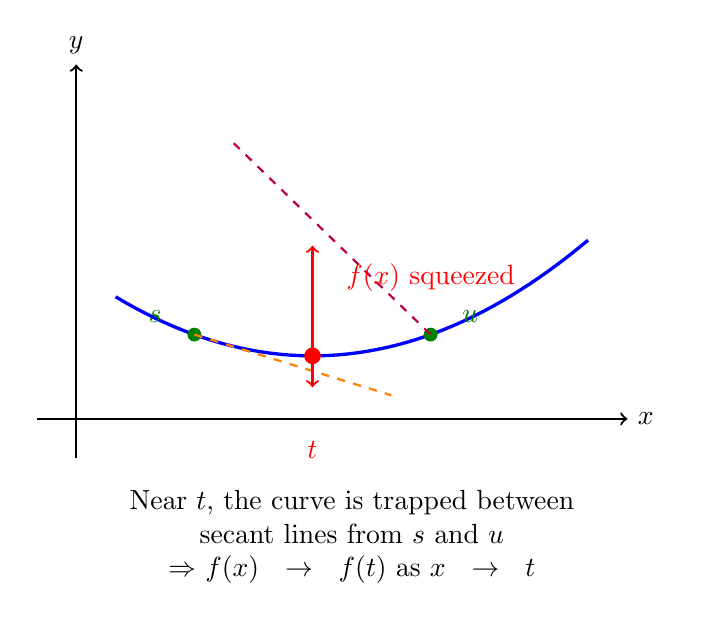
\begin{tikzpicture}[scale=1]
    \draw[thick, ->] (-0.5, 0) -- (7, 0) node[right] {$x$};
    \draw[thick, ->] (0, -0.5) -- (0, 4.5) node[above] {$y$};

    % Convex curve
    \draw[blue, very thick, domain=0.5:6.5, samples=50] plot (\x, {0.12*(\x - 3)*(\x - 3) + 0.8});

    % Point t where we want continuity
    \fill[red] (3, 0.8) circle (3pt);
    \node[red] at (3, -0.4) {$t$};

    % Points s and u flanking t
    \fill[green!50!black] (1.5, {0.12*2.25 + 0.8}) circle (2.5pt);
    \fill[green!50!black] (4.5, {0.12*2.25 + 0.8}) circle (2.5pt);
    \node[green!50!black] at (1, 1.3) {$s$};
    \node[green!50!black] at (5, 1.3) {$u$};

    % Secant lines forming a "funnel"
    \draw[orange, thick, dashed] (1.5, 1.07) -- (4, 0.3);
    \draw[purple, thick, dashed] (2, 3.5) -- (4.5, 1.07);

    % Squeeze
    \draw[<->, red, thick] (3, 0.4) -- (3, 2.2);
    \node[red] at (4.5, 1.8) {$f(x)$ squeezed};

    \node[text width=8cm, align=center] at (3.5, -1.5) {Near $t$, the curve is trapped between\\secant lines from $s$ and $u$\\$\Rightarrow$ $f(x) \to f(t)$ as $x \to t$};
\end{tikzpicture}
\end{center}

\textbf{Key idea:} The slope inequalities force $f$ to be ``sandwiched'' near any point. As $x \to t$, the secant slopes stay bounded, forcing $f(x) \to f(t)$.

\section{Part 3: Composition}

\textbf{Claim:} If $f$ is convex and $g$ is increasing and convex, then $g \circ f$ is convex.

\begin{center}
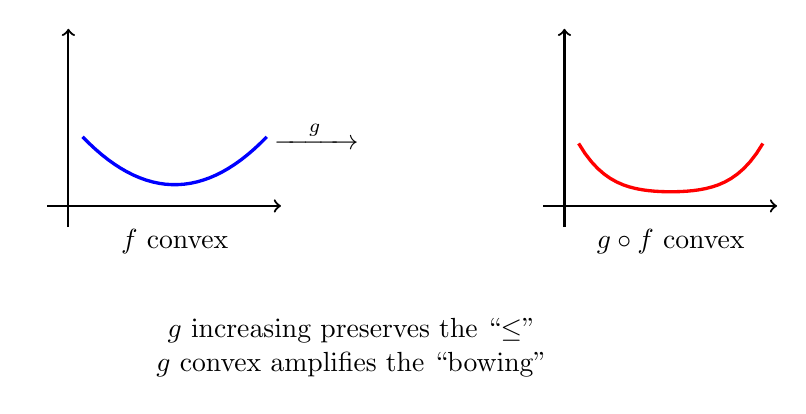
\begin{tikzpicture}[scale=0.9]
    % f is convex
    \begin{scope}[xshift=-4cm]
        \draw[thick, ->] (-0.3, 0) -- (3, 0);
        \draw[thick, ->] (0, -0.3) -- (0, 2.5);
        \draw[blue, very thick, domain=0.2:2.8, samples=30] plot (\x, {0.4*(\x - 1.5)*(\x - 1.5) + 0.3});
        \node at (1.5, -0.5) {$f$ convex};
    \end{scope}

    \node at (-0.5, 1) {$\xrightarrow{\quad g \quad}$};

    % g(f) is convex
    \begin{scope}[xshift=3cm]
        \draw[thick, ->] (-0.3, 0) -- (3, 0);
        \draw[thick, ->] (0, -0.3) -- (0, 2.5);
        \draw[red, very thick, domain=0.2:2.8, samples=30] plot (\x, {0.15*(\x - 1.5)*(\x - 1.5)*(\x - 1.5)*(\x - 1.5) + 0.15*(\x - 1.5)*(\x - 1.5) + 0.2});
        \node at (1.5, -0.5) {$g \circ f$ convex};
    \end{scope}

    \node[text width=8cm, align=center] at (0, -2) {$g$ increasing preserves the ``$\leq$''\\$g$ convex amplifies the ``bowing''};
\end{tikzpicture}
\end{center}

\textbf{Example:} $f$ convex $\implies$ $e^f$ convex (since $e^x$ is increasing and convex).

\section{Summary}

\begin{center}
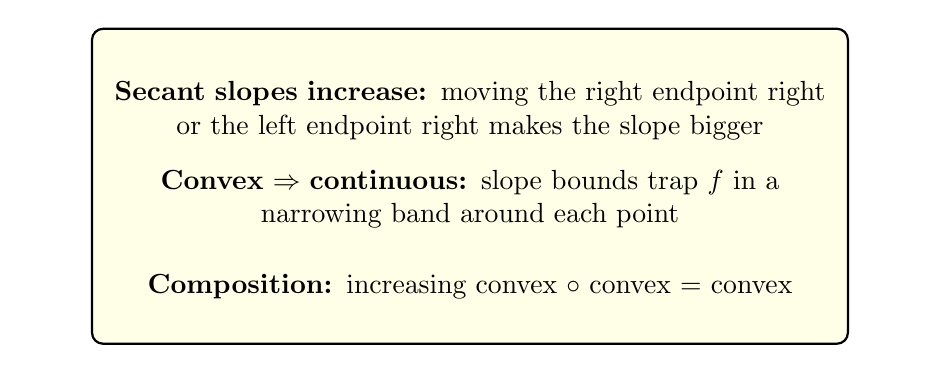
\begin{tikzpicture}[scale=0.8]
    \draw[thick, rounded corners, fill=yellow!10] (-6, -2.5) rectangle (6, 2.5);
    \node[text width=11cm, align=center] at (0, 1.2) {
        \textbf{Secant slopes increase:} moving the right endpoint right\\
        or the left endpoint right makes the slope bigger
    };
    \node[text width=11cm, align=center] at (0, -0.2) {
        \textbf{Convex $\Rightarrow$ continuous:} slope bounds trap $f$ in a\\
        narrowing band around each point
    };
    \node[text width=11cm, align=center] at (0, -1.6) {
        \textbf{Composition:} increasing convex $\circ$ convex = convex
    };
\end{tikzpicture}
\end{center}

\end{document}
